% Options for packages loaded elsewhere
\PassOptionsToPackage{unicode}{hyperref}
\PassOptionsToPackage{hyphens}{url}
%
\documentclass[
]{book}
\usepackage{lmodern}
\usepackage{amsmath}
\usepackage{ifxetex,ifluatex}
\ifnum 0\ifxetex 1\fi\ifluatex 1\fi=0 % if pdftex
  \usepackage[T1]{fontenc}
  \usepackage[utf8]{inputenc}
  \usepackage{textcomp} % provide euro and other symbols
  \usepackage{amssymb}
\else % if luatex or xetex
  \usepackage{unicode-math}
  \defaultfontfeatures{Scale=MatchLowercase}
  \defaultfontfeatures[\rmfamily]{Ligatures=TeX,Scale=1}
\fi
% Use upquote if available, for straight quotes in verbatim environments
\IfFileExists{upquote.sty}{\usepackage{upquote}}{}
\IfFileExists{microtype.sty}{% use microtype if available
  \usepackage[]{microtype}
  \UseMicrotypeSet[protrusion]{basicmath} % disable protrusion for tt fonts
}{}
\makeatletter
\@ifundefined{KOMAClassName}{% if non-KOMA class
  \IfFileExists{parskip.sty}{%
    \usepackage{parskip}
  }{% else
    \setlength{\parindent}{0pt}
    \setlength{\parskip}{6pt plus 2pt minus 1pt}}
}{% if KOMA class
  \KOMAoptions{parskip=half}}
\makeatother
\usepackage{xcolor}
\IfFileExists{xurl.sty}{\usepackage{xurl}}{} % add URL line breaks if available
\IfFileExists{bookmark.sty}{\usepackage{bookmark}}{\usepackage{hyperref}}
\hypersetup{
  pdftitle={Mekanik Kuantum},
  pdfauthor={Murthadza Aznam},
  hidelinks,
  pdfcreator={LaTeX via pandoc}}
\urlstyle{same} % disable monospaced font for URLs
\usepackage{longtable,booktabs}
\usepackage{calc} % for calculating minipage widths
% Correct order of tables after \paragraph or \subparagraph
\usepackage{etoolbox}
\makeatletter
\patchcmd\longtable{\par}{\if@noskipsec\mbox{}\fi\par}{}{}
\makeatother
% Allow footnotes in longtable head/foot
\IfFileExists{footnotehyper.sty}{\usepackage{footnotehyper}}{\usepackage{footnote}}
\makesavenoteenv{longtable}
\usepackage{graphicx}
\makeatletter
\def\maxwidth{\ifdim\Gin@nat@width>\linewidth\linewidth\else\Gin@nat@width\fi}
\def\maxheight{\ifdim\Gin@nat@height>\textheight\textheight\else\Gin@nat@height\fi}
\makeatother
% Scale images if necessary, so that they will not overflow the page
% margins by default, and it is still possible to overwrite the defaults
% using explicit options in \includegraphics[width, height, ...]{}
\setkeys{Gin}{width=\maxwidth,height=\maxheight,keepaspectratio}
% Set default figure placement to htbp
\makeatletter
\def\fps@figure{htbp}
\makeatother
\setlength{\emergencystretch}{3em} % prevent overfull lines
\providecommand{\tightlist}{%
  \setlength{\itemsep}{0pt}\setlength{\parskip}{0pt}}
\setcounter{secnumdepth}{-\maxdimen} % remove section numbering
\ifluatex
  \usepackage{selnolig}  % disable illegal ligatures
\fi
\newlength{\cslhangindent}
\setlength{\cslhangindent}{1.5em}
\newlength{\csllabelwidth}
\setlength{\csllabelwidth}{3em}
\newenvironment{CSLReferences}[2] % #1 hanging-ident, #2 entry spacing
 {% don't indent paragraphs
  \setlength{\parindent}{0pt}
  % turn on hanging indent if param 1 is 1
  \ifodd #1 \everypar{\setlength{\hangindent}{\cslhangindent}}\ignorespaces\fi
  % set entry spacing
  \ifnum #2 > 0
  \setlength{\parskip}{#2\baselineskip}
  \fi
 }%
 {}
\usepackage{calc}
\newcommand{\CSLBlock}[1]{#1\hfill\break}
\newcommand{\CSLLeftMargin}[1]{\parbox[t]{\csllabelwidth}{#1}}
\newcommand{\CSLRightInline}[1]{\parbox[t]{\linewidth - \csllabelwidth}{#1}\break}
\newcommand{\CSLIndent}[1]{\hspace{\cslhangindent}#1}

\title{Mekanik Kuantum}
\author{Murthadza Aznam}
\date{2020-12-31}

\begin{document}
\frontmatter
\maketitle

\mainmatter
\hypertarget{prakata}{%
\chapter*{Prakata}\label{prakata}}
\addcontentsline{toc}{chapter}{Prakata}

Placeholder

\hypertarget{dorongan-projek}{%
\section*{Dorongan Projek}\label{dorongan-projek}}
\addcontentsline{toc}{section}{Dorongan Projek}

\hypertarget{tentang-penulis}{%
\section*{Tentang Penulis}\label{tentang-penulis}}
\addcontentsline{toc}{section}{Tentang Penulis}

\hypertarget{tentang-buku}{%
\section*{Tentang Buku}\label{tentang-buku}}
\addcontentsline{toc}{section}{Tentang Buku}

\hypertarget{malapetaka-ultralembayung}{%
\chapter{Malapetaka Ultralembayung}\label{malapetaka-ultralembayung}}

Catatan-catatan sejarah sains menulis bahawa kegiatan kajian dunia
kuantum bermula dengan kajian terhadap sinaran yang dipancarkan oleh
bintang-bintang. Agak hairan bagaimana butiran-butiran bintang yang
bertaburan di langit malam yang hakikatnya sebesar ribuan gunung-ganang
itu mampu memberi kita ilham tentang dunia kuantum yang lebih kecil
daripada pasir. Cahayalah yang menghubungkan dunia sebesar-besar bintang
dengan dunia sekecil-kecil zarah. Cahayalah juga yang membawa kita
meneroka dua dunia baharu fizik yakni dunia kuantum dan dunia kenisbian
seolah-olah cahaya ialah penyuluh harapan kepada fizikawan sekalian alam
ketika jalan menjadi suram.

\hypertarget{sinaran-jasad-hitam}{%
\section{Sinaran Jasad Hitam}\label{sinaran-jasad-hitam}}

Jasad hitam ialah suatu jasad yang akan menyerap semua panjang gelombang
cahaya dengan sempurna tanpa pantulan. Jasad ini akan memancarkan juga
kesemua panjang gelombang apabila berada dalam keseimbangan haba. Kata
kuncinya di sini ialah ia memancarkan kesemua panjang gelombang cahaya
daripada sependek-pendek gamma sehinggalah sepanjang-panjang radio.
Bintang-bintang di langit memiliki ciri ini.

Cahaya yang dipancarkan oleh bintang-bintang ini membawa bersamanya
tenaga. Jumlah tenaga yang dikeluarkan oleh setiap bintang mematuhi
Hukum Stefan--Boltzmann.

\BeginKnitrBlock{definition}\iffalse{-91-72-117-107-117-109-32-83-116-101-102-97-110-45-45-66-111-108-116-122-109-97-110-110-93-}\fi{}

\protect\hypertarget{def:mu-def-01}{}{(\#def:mu-def-01) \iffalse (Hukum
Stefan--Boltzmann) \fi{} }Jumlah tenaga, \(E\), yang dikeluarkan oleh
bintang adalah berkadaran dengan suhunya, \(T\), \begin{equation}
  E = \sigma T^4,
\end{equation} dengan maksud bahawa, \begin{equation*}
\begin{split}
    E & = \text{tenaga},\\
    T & = \text{suhu bintang},\\
    \sigma & = \text{pemalar Stefan--Boltzmann,}\\
    & = 5.6704\times 10^{-8}\text{W}\cdot\text{s}^{-1}\cdot\text{K}^{-4}.\\
\end{split}
\end{equation*} \EndKnitrBlock{definition}

Tenaga yang diperihalkan dalam Hukum Stefan--Boltzmann ini adalah jumlah
tenaga yang dibawa oleh semua frekuensi cahaya. Ada sebahagian cahaya
yang bersinar lebih kuat berbanding cahaya yang lain. Lazimnya, cahaya
yang panjang (seperti radio) dan cahaya yang pendek (seperti sinaran
gamma) tidak dipancarkan dengan banyak. Kebanyakan cahaya yang
disinarkan oleh setiap satu jasad berada di antara dua nilai yang
disebutkan itu.

\begin{figure}
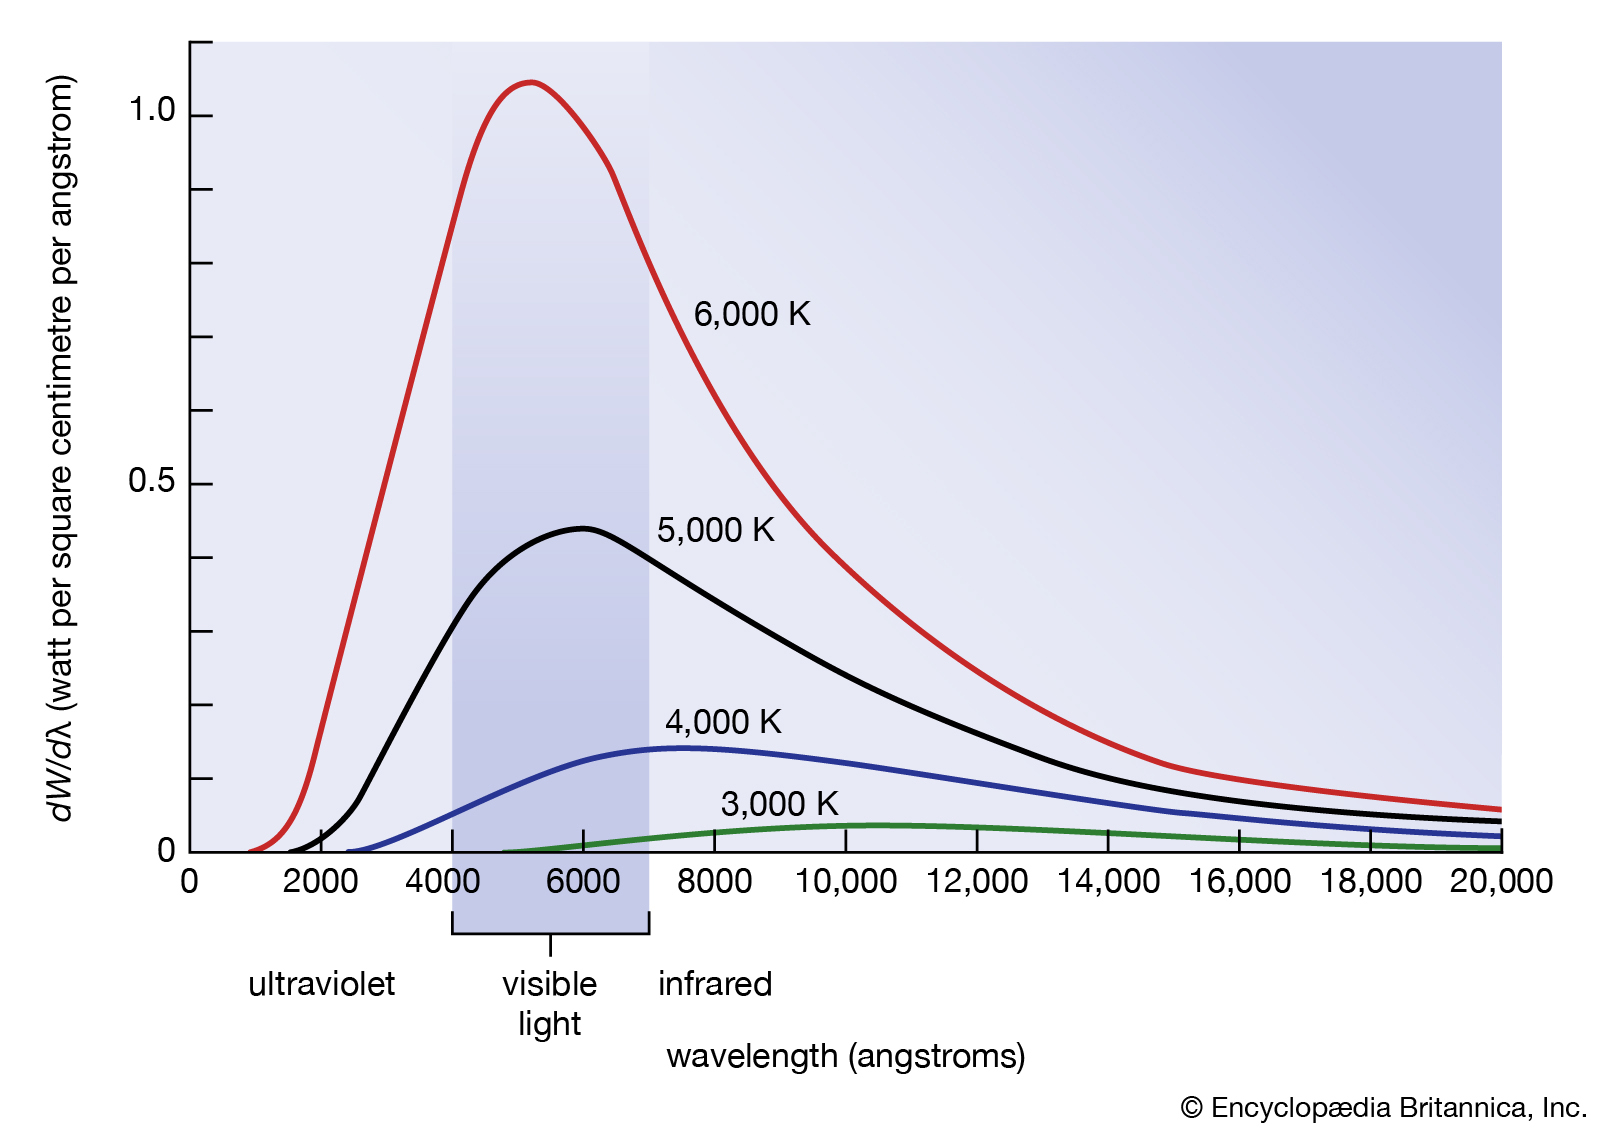
\includegraphics[width=400px]{./gambar/ultra/jasadhitam} \caption{Graf keamatan cahaya melawan panjang gelombang yang dipancarkan suatu bintang.}\label{fig:mu-jasad}
\end{figure}

Rajah @ref(fig:mu-jasad) menunjukkan taburan cahaya yang dipancarkan
oleh sesuatu bintang mengikut panjang gelombang cahaya. Puncak lengkung
itu menunjukkan cahaya mana yang paling banyak dikeluarkan. Puncak itu
semakin menghampiri kiri jika suhu bintang semakin panas.

Hal ini yang menentukan warna bintang tersebut. Jika bintangnya panas,
maka puncak lengkungnya akan ke arah warna biru. Jika bintangnya sejuk,
maka puncak lengkungnya akan ke arah warna merah. Kita boleh lihat
perbezaan warna ini dengan mata kasar jika kita teliti. Puncak graf
tersebut mematuhi Hukum Sesaran Wien.

\textbackslash begin\{figure\}
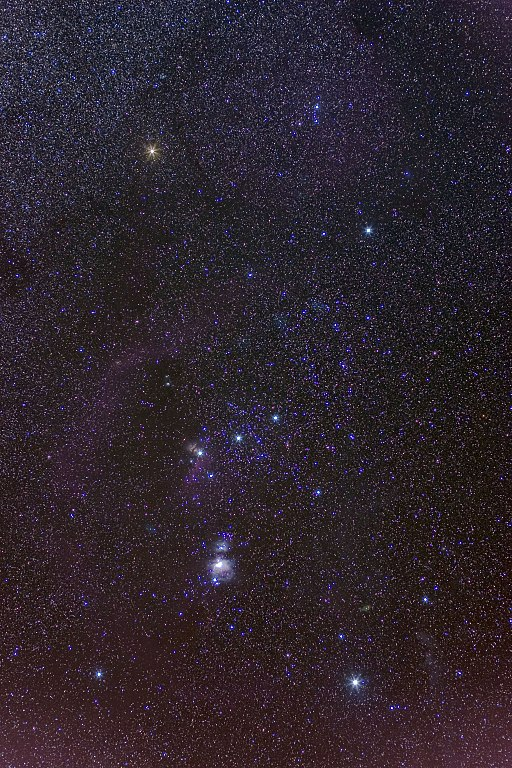
\includegraphics[height=400px]{./gambar/ultra/belantik}
\textbackslash caption\{Buruj Belantik. Bintang Betelguese (kiri atas)
berwarna merah manakala bintang Rigel (kanan bawah) berwarna biru. Dari
sini kita boleh simpulkan bahawa bintang Rigel lebih panas berbanding
bintang Betelguese. Karya:
\href{https://commons.wikimedia.org/wiki/File:Orion_3008_huge.jpg}{Mouser},
CC BY--SA 3.0.\}\label{fig:mu-belantik} \textbackslash end\{figure\}

\BeginKnitrBlock{definition}\iffalse{-91-72-117-107-117-109-32-83-101-115-97-114-97-110-32-87-105-101-110-93-}\fi{}

\protect\hypertarget{def:mu-def-02}{}{(\#def:mu-def-02) \iffalse (Hukum
Sesaran Wien) \fi{} }Panjang gelombang puncak sinaran jasad hitam,
\(\lambda_p\), adalah berkadaran songsang dengan suhu bintang tersebut,
\(T\), \begin{equation}
    \lambda_p = \frac{W}{T},
\end{equation} dengan maksud bahawa, \begin{equation*}
\begin{split}
    \lambda_p & = \text{panjang gelombang puncak,} \\
    T & = \text{suhu jasad hitam,} \\
    W & = \text{pemalar Wien,} \\
    & = 2.8978\times 10^{-3}\text{m}\cdot\text{K}.\\
\end{split}
\end{equation*} \EndKnitrBlock{definition}

Pemerihalan jumlah tenaga dan nilai tenaga puncak itu cukup mantap.
Namun, pencarian ahli fizik belum selesai kerana mereka ingin tahu
persamaan apakah yang boleh menghasilkan graf tersebut, bukan sekadar
jumlah tenaga atau puncaknya sahaja.

Hukum Stefann--Boltzmann hanya mampu menerangkan jumlah tenaga bintang.
Hukum Wien pula hanya menyatakan di mana letaknya puncak graf tersebut.
Kedua-duanya tidak mampu menerangkan lengkungan graf tersebut.

\hypertarget{sec:wien-rayleigh-jeans}{%
\section{Cubaan Wein, Rayleigh dan
Jeans}\label{sec:wien-rayleigh-jeans}}

Pada tahun 1897, seorang fizikawan Jerman bernama Wilhelm Wien cuba
menyelesaikan masalah ini dengan membina persamaan sinaran jasad hitam
berdasarkan pengetahuan keelektromagnetan sedia ada. Persamaan beliau
dikenali sebagai Hukum Taburan Wien. Namun, persamaan beliau hanya mampu
meramalkan tenaga untuk cahaya-cahaya pendek dan ia tidak meramalkan
dengan tepat untuk cahaya-cahaya panjang. Oleh itu, ia juga dikenali
sebagai Penghampiran Wien.

\BeginKnitrBlock{definition}\iffalse{-91-72-117-107-117-109-32-84-97-98-117-114-97-110-32-87-105-101-110-32-47-32-80-101-110-103-104-97-109-112-105-114-97-110-32-87-105-101-110-93-}\fi{}

\protect\hypertarget{def:mu-def-03}{}{(\#def:mu-def-03) \iffalse (Hukum
Taburan Wien / Penghampiran Wien) \fi{} }Ketumpatan tenaga cahaya, \(U\)
adalah berkadaran eksponensial dengan suhu dan panjang gelombang,
\(\text{exp}\Big\{-\frac{1}{\lambda T}\Big\}\), dan berkadaran songsang
dengan suhu berkuasa lima, \(\lambda^5\), \begin{equation}
U(\lambda,T) = \frac{ae^{-\frac{b}{\lambda T}}}{\lambda^5},
\end{equation} dengan maksud bahawa, \begin{equation*}
\begin{split}
U(\lambda,T) & = \text{ketumpatan tenaga cahaya},\\
\lambda & = \text{panjang gelombang cahaya},\\
T & = \text{suhu bintang},\\
a,b & = \text{pemalar}.\\
\end{split}
\end{equation*} \EndKnitrBlock{definition}

Pada sekitar tahun 1900-an, ahli fizik Lord Rayleigh dan James Jeans
mengemukakan persamaan mereka yang disangka boleh menyelesaikan masalah
ini. Mereka menganggap bahawa jasad hitam itu terdiri daripada
pengayun-pengayun klasik. Hasilnya, persamaan Rayleigh--Jeans hanya
mampu meramalkan tenaga untuk cahaya-cahaya panjang sahaja.

\BeginKnitrBlock{definition}\iffalse{-91-72-117-107-117-109-32-82-97-121-108-101-105-103-104-45-45-74-101-97-110-115-93-}\fi{}

\protect\hypertarget{def:mu-def-04}{}{(\#def:mu-def-04) \iffalse (Hukum
Rayleigh--Jeans) \fi{} }Ketumpatan tenaga cahaya, \(U\), adalah
berkadaran terus dengan suhu bintang \(T\) dan berkadaran songsang
dengan panjang gelombang cahaya kuasa empat, \(\lambda^4\),
\begin{equation}
U\left(\lambda,T\right) = 8\pi\frac{k_BT}{\lambda^4},
\end{equation} dengan maksud bahawa, \begin{equation*}
\begin{split}
U & = \text{ketumpatan tenaga cahaya},\\
k_B & = \text{pemalar Boltzmann},\\
&= 1.380649\times 10^{-23} \text{J}\cdot\text{K}^{-1},\\
\lambda & = \text{panjang gelombang cahaya},\\
T & = \text{suhu bintang}.\\
\end{split}
\end{equation*} \EndKnitrBlock{definition}

\BeginKnitrBlock{proof}\iffalse{-91-75-97-101-100-97-104-32-77-101-109-112-101-114-111-108-101-104-32-80-101-114-115-97-109-97-97-110-32-82-97-121-108-101-105-103-104-45-45-74-101-97-110-115-93-}\fi{}

\iffalse{} {BUKTI (Kaedah Memperoleh Persamaan Rayleigh--Jeans) }
\fi{}Bagi memperoleh persamaan Rayleigh--Jeans (Hukum
@ref(def:mu-def-01)), kita akan bermula dengan menakrif jumlah tenaga
yang dimiliki oleh setiap pengayun serta menakrifkan jumlah pengayun.

\textbf{USUL 1}: Pengayun-pengayun Rayleigh--Jeans mematuhi teorem
pemetakan sama, iaitu semua bentuk tenaga akan memiliki jumlah purata
yang sama. Sistem pengayun Rayleigh--Jeans memiliki dua bentuk tenaga
iaitu tenaga kinetik, \(E_k\), dan tenaga upaya, \(E_v\) dan
masing-masing mempunyai nilai \(\frac{1}{2}{k_BT}\),
\[E_k = E_v = \frac{1}{2}{k_BT}.\]

Maka, tenaga setiap pengayun tersebut ialah \(k_BT\), \begin{equation}
\sum E = E_k + E_v = \frac{1}{2}{k_BT} + \frac{1}{2}{k_BT} =k_BT (\#eq:mu-0)
\end{equation}

\textbf{USUL 2}: Ketumpatan pengayun ialah berkadaran dengan frekuensi
kuasa dua \(f^2\), \begin{equation}
n(f) = \frac{8\pi f^2}{c^3}.(\#eq:mu-1)
\end{equation} Nilai \(n(f)\) ini dikenali sebagai nilai Jeans.

Oleh itu, tenaga yang dibawa oleh setiap frekuensi cahaya,
\(U\left(\lambda,T\right)\), boleh diperoleh sebagai hasil darab nilai
Jeans (pers. @ref(eq:mu-1)) dengan tenaga pengayun (pers.
@ref(eq:mu-0)), \begin{equation}
U\left(\lambda,T\right) = n\left(f\right)k_BT.
(\#eq:mu-2)
\end{equation}

Persamaan Rayleigh--Jeans (Hukum @ref(def:mu-def-01)) memerihalkan
tenaga cahaya dalam bentuk panjang gelombang \(\lambda\), maka nilai
Jeans tersebut perlu diterjemahkan dalam bentuk panjang gelombang. Hal
ini mudah kerana kita tahu hubungan antara frekuensi dan panjang
gelombang ialah, \begin{equation}
f = \frac{c}{\lambda},(\#eq:mu-3)
\end{equation} dan kita lakukan pembezaan siap-siap, \begin{equation}
\frac{\text{d}f}{\text{d}\lambda} = \frac{-c}{\lambda^2}.
(\#eq:mu-3a)
\end{equation}

Fungsi nilai Jeans pula boleh ditukar menggunakan perhubungan ini,
\begin{equation}
n\left(\lambda\right) = n(f)\left|\frac{\text{d}{f}}{\text{d}{\lambda}}\right|.
(\#eq:mu-4)
\end{equation} Fungsi pembezaan
\(\frac{\text{d}{f}}{\text{d}{\lambda}}\) dimutlakkan sebab nilai Jeans
ialah jumlah pengayun. Jumlah benda fizikal tidak boleh berada dalam
julat negatif.

Dengan memasukkan pers. @ref(eq:mu-1) dan pers. @ref(eq:mu-3a) ke dalam
pers. @ref(eq:mu-4), \begin{equation}
n(\lambda) = \left(\frac{8\pi f^2}{c^3}\right)\left|\frac{-c}{\lambda^2}\right|.
  (\#eq:mu-5)
\end{equation} Kemudian, pembolehubah \(f\) perlu diganti dengan
perkaitan dalam pers. @ref(eq:mu-3), \begin{equation}
n(\lambda) = \left(\frac{8\pi}{c^3}\left(\frac{c}{\lambda}\right)^2\right)\left|\frac{-c}{\lambda^2}\right|.
  (\#eq:mu-6)
\end{equation} Maka, nilai \(n(\lambda)\) ialah, \begin{equation}
n\left(\lambda\right) = \frac{8\pi}{\lambda^4}.
(\#eq:mu-7)
\end{equation}

Maka, langkah terakhir kita ialah dengan menggunakan pers. @ref(eq:mu-7)
untuk menyelesaikan pers. @ref(eq:mu-2) di awal kaedah ini tadi,
\begin{equation}
U\left(\lambda,T\right) = 8\pi\frac{k_BT}{\lambda^4}.
\end{equation} Inilah persamaan Rayleigh--Jeans yang ingin diperolehi.
\EndKnitrBlock{proof}

Hasil daripada persamaan Rayleigh--Jeans ialah suatu graf yang
menghampiri sifar untuk panjang gelombang yang panjang, tetapi akan
menghampiri infiniti untuk panjang gelombang pendek. Hakikat ini nyata
bagi yang celik Matematik kerana persamaan Rayleigh--Jeans ialah suatu
fungsi salingan, \(\frac{1}{x}\), berkuasa 4.

Maknanya, menurut persamaan ini, bintang akan memancarkan cahaya
berpanjang gelombang pendek dengan tenaga yang tidak terhingga! Perkara
ini adalah mustahil kerana ia melanggar hukum keabadian tenaga
seolah-olah jisim yang terbatas boleh menghasilkan tenaga yang tidak
terbatas.

Kejadian ini lazimnya diberi nama ``Malapetaka Ultralembayung'' kerana
sifat gelombang ultralembayung yang pendek panjang gelombangnya.
Walaupun tiada malapetaka sebenar yang meragut mana-mana nyawa, nama itu
sedap disebut dan selari dengan naluri manusia yang sukakan cerita
menarik maka ia melekat dalam lidah para fizikawan.

\begin{figure}

{\centering 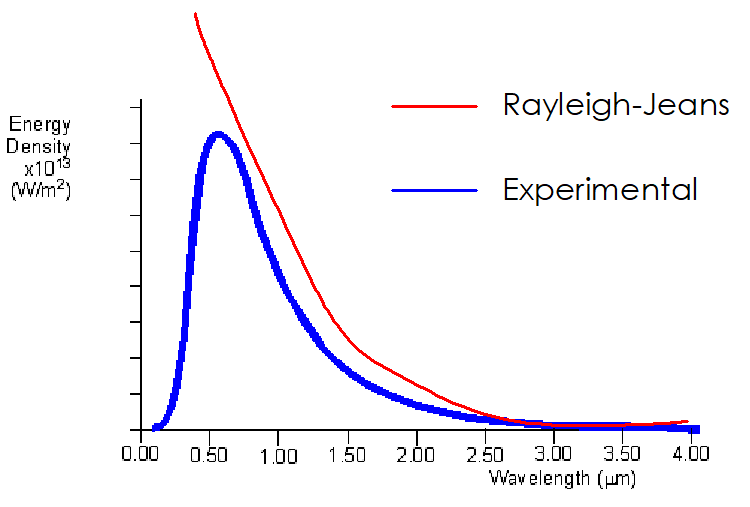
\includegraphics[width=500px]{./gambar/ultra/Rayleigh} 

}

\caption{Persamaan Rayleigh--Jeans meramalkan tenaga tidak terhingga untuk cahaya-cahaya pendek. Hal ini tidak masuk akal.}\label{fig:unnamed-chunk-2}
\end{figure}

\BeginKnitrBlock{istilah}

\textbf{Dari segi bahasa}: Dalam bahasa Melayu, perkataan
\emph{lembayung} merujuk kepada warna ungu kejinggaan yang boleh dilihat
ketika langit senja atau ketika matahari rendah. Imbuhan \emph{ultra-}
pula ialah imbuhan daripada bahasa Inggeris yang menunjukkan sifat
tersebut melangkaui sifat yang biasa.

\textbf{Dari segi istilah}: Dalam fizik, istilah \emph{ultralembayung}
merujuk kepada warna cahaya yang bertenaga tinggi dalam julat 10 ke 400
nanometer yang lebih pendek daripada warna lembayung (sekitar 400
nanometer).

\EndKnitrBlock{istilah}

\hypertarget{sec:postulat-planck}{%
\section{Postulat Planck Tentang Sekuantum
Tenaga}\label{sec:postulat-planck}}

Penyelesaian kepada masalah ini diberikan oleh Max Planck dengan dua
postulat yang dibawanya. Postulat-postulat ini mengandaikan bahawa
cahaya bukanlah selanjar seperti gelombang tetapi seperti berketul-ketul
seperti zarah. Ternyata, persamaan yang muncul dari postulat ini
menghasilkan graf yang selari dengan hasil cerapan.

\textbf{POSTULAT 1}: Tenaga, \(\varepsilon\), yang dipancarkan oleh
pengayun-pengayun dalam jasad hitam itu bergantung kepada frekuensi
cahaya, \(f\), \[\varepsilon = hf.\] (\(h\) ialah pemalar)

\textbf{POSTULAT 2}: Tenaga, \(\varepsilon_n\), yang dipancarkan oleh
pengayun-pengayun dalam jasad hitam mempunyai tahap tenaga berhasil
darab integer, \[\varepsilon_n = n\varepsilon,\] \[n=1,2,3,\cdots\]

Adapun begitu, perkara ini bertentangan dengan pandangan ahli fizik
tentang cahaya yang dipegang pada zaman itu. Selama ini, cahaya
dipandang sebagai suatu gelombang selanjar yang selari dengan persamaan
Maxwell. Postulat yang diusulkan itu menatijahkan bahawa cahaya itu
sifatnya berketul-ketul. Satu ketul cahaya inilah yang disebut satu
kuantum cahaya.

Max Planck sendiri menolak postulat yang dikemukakannya. Postulat
tersebut hanyalah cubaannya sahaja dan mendapati ia selari dengan hasil
cerapan. Baginya, ia adalah ralat dalam dunia Matematik dan ia akan
dapat diperbetulkan di kemudian hari.

Namun begitu, dua postulat ini kekal sehingga hari ini setelah banyak
ujikaji lain mengesahkannya. Fizikawan mendapati cahaya mempunyai
kedua-dua sifat gelombang dan zarah. Pemilikan dua sifat ini dipanggil
kedualan gelombang--zarah dan sifat ini adalah asas kepada Mekanik
Kuantum. Pemalar \(h\) itu kini dikenali sebagai Pemalar Planck.

\BeginKnitrBlock{definition}\iffalse{-91-72-117-107-117-109-32-80-108-97-110-99-107-93-}\fi{}

\protect\hypertarget{def:mu-def-05}{}{(\#def:mu-def-05) \iffalse (Hukum
Planck) \fi{} }Ketumpatan tenaga cahaya, \(U\), adalah berkadaran
songsang terhadap panjang gelombang kuasa 5, \(\lambda^5\), dan
berkadaran songsang terhadap eksponen \(\lambda T\) tolak satu,
\(\text{exp}\Big\{\frac{1}{\lambda T}\Big\} - 1\), \begin{equation}
U(\lambda, T)=\frac{8\pi hc}{\lambda^5}\frac{1}{e^{\frac{hc}{\lambda k_BT}}-1}
\end{equation} dengan maksud bahawa, \begin{equation*}
\begin{split}
U(\lambda, T) & = \text{ketumpatan tenaga},\\
\lambda & = \text{panjang gelombang cahaya},\\
T & = \text{suhu bintang},\\
h & = \text{pemalar Planck},\\
& = 6.62607015\times 10^{-34}\text{J}\cdot\text{s},\\
c & = \text{kelajuan cahaya},\\
& = 2.99792458\times 10^8 \text{m}\cdot\text{s}^{-1},\\
k_B & = \text{pemalar Boltzmann},\\
& = 1.380649\times 10^{-23} \text{J}\cdot\text{K}^{-1}.\\
\end{split}
\end{equation*} \EndKnitrBlock{definition}

(Kaedah Memperoleh Persamaan Planck) Bagi memperoleh persamaan Planck
(Hukum @ref(def:mu-def-05)), kita akan bermula dengan menakrif jumlah
tenaga yang dimiliki oleh setiap pengayun serta menakrifkan jumlah
pengayunnya.

\textbf{USUL 1}: Pengayun-pengayun Planck mempunyai tenaga,
\(\varepsilon_n\), yang berkadaran terus terhadap frekuensi, \(f\), dan
berpekali integer, \(n\), seperti yang dijelaskan dalam dua postulat
Planck, \begin{equation}
\varepsilon_n = nhf
(\#eq:mu-10)
\end{equation}

\textbf{USUL 2}: Jumlah pengayun dalam jasad hitam mematuhi taburan
Maxwell--Boltzmann, \begin{equation}
N(n)= N_0\exp\Big\{\frac{-\varepsilon_n}{k_BT}\Big\},
(\#eq:mu-11)
\end{equation} dengan maksud bahawa, \begin{equation*}
\begin{split}
N(n) &= \text{jumlah pengayun yang mempunyai tenaga $\varepsilon_n$},\\
N_0 &= \text{sejenis pemalar}\\
\varepsilon_n &= nhf\\
k_B &= \text{pemalar Boltzmann}.
\end{split}
\end{equation*} Tatatanda
\(\text{exp}\Big\{\frac{-\varepsilon_n}{k_BT}\Big\}\) digunakan untuk
menggantikan \(e^{\frac{-\varepsilon_n}{k_BT}}\) supaya pecahan dalam
kuasa eksponen itu lebih jelas kelihatan tetapi kedua-duanya mempunyai
maksud yang sama.

Oleh itu, purata tenaga, \(\overline{\varepsilon}\), yang dipancarkan
oleh jasad hitam boleh diungkapkan sebagai hasil jumlah tenaga yang
dibawa oleh semua pengayun, \(N(n)\varepsilon_n\), dibahagikan dengan
jumlah pengayun, \(N(n)\), \begin{equation}
\overline{\varepsilon} = \frac{\sum_{n=0}^{\infty}N(n)\varepsilon_n}{\sum_{n=0}^{\infty}N(n)}.
(\#eq:mu-12)
\end{equation}

Perhatikan bagaimana penjumlahan ini dilaksanakan. Purata tenaga
tersebut dijumlahkan menggunakan penjumlahan (\(\sum\)) dan bukannya
pengamiran (\(\int\)). Cuba ingat semula kelas kalkulus tentang makna
pengamiran serta perbezaannya dengan penjumlahan.

Pengamiran hanya sah digunakan sekiranya tiada rongga dalam nilai \(n\).
Maksudnya, semua nilai dalam julat \([n_1, n_2]\) mempunyai makna. Sifat
ketiadaan rongga ini disebut sebagai sifat selajar.

Sebaliknya, penjumlahan hanya sah digunakan sekiranya terdapat rongga
dalam nilai \(n\). Maksudnya, nilai pertama dan nilai kedua dipisahkan
oleh satu nilai tertentu, katakanlah \(\Delta n\). Dalam kes ini,
\(n=1\) dan \(n=2\) dipisahkan oleh \(\Delta n = 1\). Natijahnya, nilai
perantara seperti \(n=0.5\) tiada makna dalam penjumlahan ini. Sifat set
nilai yang berongga ini disebut sebagai sifat diskret.

Penggunaan penjumlahan dalam pers. @ref(eq:mu-12) menonjolkan lagi sifat
kediskretan cahaya yang kita sebut berketul-ketul tadi. Ia selari dengan
postulat keduanya yang mengatakan bahawa pekali \(n\) ialah nilai
integer.

Pers. @ref(eq:mu-12) boleh dikembangkan mengikut takrif nilai \(N(n)\)
dan \(\varepsilon_n\) yang diberikan sebelum ini, \begin{equation}
\overline{\varepsilon} = \frac{\sum N_0\exp\Big\{\frac{-nhf}{k_BT}\Big\} nhf}{\sum N_0\exp\Big\{\frac{-nhf}{k_BT}\Big\}}.
(\#eq:mu-13)
\end{equation}

Pekali \(N_0\) dan \(hf\) pula boleh difaktorkan keluar kerana malar
dalam hal penjumlahan ini. Kemudian, \(N_0\) di atas dan di bawah boleh
dipotong. Pemalar \(\frac{-hf}{k_BT}\) dalam
\(\exp\Big\{\frac{-nhf}{k_BT}\Big\}\) akan digantikan dengan \(k\).
Pers. @ref(eq:mu-12) kini adalah,
\[\overline{\varepsilon} = hf\frac{\sum n e^{nk}}{\sum e^{nk}}\] Apabila
dikembangkan penjumlahannya, kita akan dapat, \begin{equation}
\overline{\varepsilon} = hf\lim_{N\to\infty}\frac{(0)e^{0k} + (1)e^{1k} + (2)e^{2k} + (3)e^{3k}+\dots+Ne^{Nk}}{e^{0k}+e^{1k}+e^{2k}+e^{3k}+\dots+e^{Nk}}.
(\#eq:mu-14)
\end{equation}

Mari kita perhatikan setiap satu sebutan dalam pecahan tersebut. Untuk
nilai pengangka, sebutan pertamanya ialah sifar maka hanya tinggal
sebutan berpekali integer sahaja. Kemudian kita dapati setiap satu
sebutan di bahagian atas tersebut mengongsi sebutan sepunya, iaitu
\(e^k\). Maka, nilai pengangka tersebut akan menjadi
\[\lim_{N\to\infty}e^k(1+2e^k+3e^{2k}+\cdots+Ne^{(N-1)k}).\] Untuk nilai
pembawah pula, sebutan pertamanya ialah \(e^{0k}=e^0=1\) dan
sebutan-sebutan lain tidak mengalami perubahan.

Ini persamaan baharu kita, \begin{equation}
\overline{\varepsilon} = hfe^k \lim_{N\to\infty} \frac{1+2e^k+3e^{2k}+\dots+Ne^{(N-1)k}}{1+e^k+e^{2k}+e^{3k}+\dots+x^{Nk}}
(\#eq:mu-15)
\end{equation}

Pers. @ref(eq:mu-15) menonjolkan dua jenis siri, iaitu siri geometri
yang menjadi nilai pembawah pecahan tersebut, dan pembezaan siri
geometri yang menjadi nilai pengangkanya.

\BeginKnitrBlock{theorem}\iffalse{-91-83-105-114-105-32-71-101-111-109-101-116-114-105-93-}\fi{}

\protect\hypertarget{thm:mu-thm-01}{}{(\#thm:mu-thm-01) \iffalse (Siri
Geometri) \fi{} }Jika \(x\) dalam
\(a + ax + ax^2 + ax^3 + \cdots + ax^N\) mempunyai ciri \(-1<x<1\) dan
\(N\to\infty\), maka siri geometrinya adalah,
\[\lim_{N\to\infty}\sum_{n=0}^N ax^n = a\frac{1}{1-x}.\] (Dipetik dari
\protect\hyperlink{ref-spiegel2009}{Spiegel, Lipschutz, and Liu 2009},
contoh 21.5) \EndKnitrBlock{theorem}
\BeginKnitrBlock{theorem}\iffalse{-91-80-101-109-98-101-122-97-97-110-32-83-105-114-105-32-71-101-111-109-101-116-114-105-93-}\fi{}
\protect\hypertarget{thm:mu-thm-02}{}{(\#thm:mu-thm-02)
\iffalse (Pembezaan Siri Geometri) \fi{} }Pembezaan siri geometri
terhadap \(x\) adalah
\[\frac{\text{d}}{\text{d}x}\sum_{n=0}^{N}ax^n = \sum_{n=0}^{N} anx^{n-1},\]
dengan jumlahnya ialah
\[\lim_{N\to\infty}\sum_{n=0}^{N} anx^{n-1} = a\frac{1}{(1-x)^2}.\]
(Dipetik dari \protect\hyperlink{ref-Mayer2006}{Mayer 2006}, contoh
12.18) \EndKnitrBlock{theorem} Nilai \(e^{nk}\) dalam pers.
@ref(eq:mu-15) menepati syarat petua @ref(thm:mu-thm-01) dan
@ref(thm:mu-thm-02) kerana \(-1<e^{nk}<1\). Maka, kedua-dua petua ini
boleh digunakan. Ganti sahaja \(a=1\) dan \(x=e^k\). Lalu, kita akan
peroleh, \begin{equation}
\overline{\varepsilon} = hfe^k\frac{(1-e^k)^{1}}{(1-e^k)^{2}},
(\#eq:mu-16)
\end{equation} yang setara dengan, \begin{equation}
\overline\varepsilon= hf\frac{1}{\frac{1}{e^k}-1}.
(\#eq:mu-17)
\end{equation} Disebabkan \(k\) ialah \(\frac{-hf}{k_BT}\), maka
\(\frac{1}{e^k} = e^{\frac{hf}{k_BT}}\).

\textbf{USUL 3}: Ketumpatan pengayun Planck mematuhi Nilai Jeans,
\begin{equation}
n(f) = \frac{8\pi f^2}{c^3}.(\#eq:mu-18)
\end{equation}

Ketumpatan tenaga, \(U\) ialah hasil darab nilai Jeans dan pers.
@ref(eq:mu-17), \begin{equation}
U = n(f)\overline{\varepsilon} = \frac{8\pi f^2}{c^3}\frac{hf}{e^{\frac{hf}{k_BT}}-1}
(\#eq:mu-19)
\end{equation} Menggunakan kaedah yang serupa dalam pers. @ref(eq:mu-4)
sehingga pers.@ref(eq:mu-7) untuk menukarkan bentuk frekuensi menjadi
bentuk panjang gelombang, kita akan peroleh persamaan Planck:
\begin{equation}
U=\frac{8\pi hc}{\lambda^5}\frac{1}{e^{\frac{hc}{\lambda k_BT}}-1}
\end{equation}

\hypertarget{sec:kesinambungan}{%
\section{Kesinambungan Persamaan Planck dengan Usaha
Sebelumnya}\label{sec:kesinambungan}}

Meskipun hanya usaha Planck sahaja yang mampu menerangkan lengkung jasad
hitam secara menyeluruh, usaha-usaha sebelumnya hanya mampu menerangkan
sebahagian sahaja daripada lengkung tersebut. Jika begitu, maknanya
persamaan Planck boleh diubah agar menyerupai persamaan-persamaan ini
dengan meletakkan syarat-syarat tertentu.

Ada empat hukum yang dibangunkan sebelum Max Planck. Yang pertama ialah
hukum Stefan--Boltzmann (Hukum @ref(def:mu-def-01)) yang menerangkan
jumlah tenaga yang disinarkan oleh bintang. Yang kedua ialah hukum
sesaran Wien (Hukum @ref(def:mu-def-02)) yang menerangkan puncak
lengkung. Yang ketiga ialah hukum taburan Wien (Hukum
@ref(def:mu-def-03)) yang menerangkan lengkung jasad hitam pada panjang
gelombang pendek. Yang keempat ialah hukum Rayleigh--Jeans (Hukum
@ref(def:mu-def-04)) yang menerangkan lengkung jasad hitam pada panjang
gelombang panjang.

Kita akan cuba memperoleh setiap satu daripadanya menggunakan Hukum
Planck mengikut turutan tersebut.

\hypertarget{sec:planck-stefan-boltzmann}{%
\subsection{Kaedah Memperoleh Hukum Stefan--Boltzmann Daripada Hukum
Planck}\label{sec:planck-stefan-boltzmann}}

Hukum Stefan--Boltzmann memerihalkan jumlah tenaga yang disinarkan oleh
suatu bintang. Hal ini sama seperti mencari luas di bawah lengkung.
Maknanya kita perlu kamirkannya terhadap panjang gelombang.

\textbf{USUL 1}: Luas bawah lengkung ialah hasil kamiran Hukum Planck
terhadap panjang gelombang dari sifar ke infiniti, \begin{equation}
E = \int_0^\infty \frac{8\pi hc}{\lambda^5}\frac{1}{e^{\frac{hc}{\lambda k_BT}}-1} \text{d}\lambda.
(\#eq:mu-20)
\end{equation}

\textbf{USUL 2}: Pembolehubah \(x\) ditakrifkan sebagai,
\begin{equation}
x = \frac{hc}{\lambda k_BT},
(\#eq:mu-21)
\end{equation} maka, \begin{equation}
\lambda = \frac{hc}{xk_BT},
(\#eq:mu-22)
\end{equation} dan, \begin{equation}
\text{d}\lambda = \text{d}x \frac{hc}{x^2k_BT}.
(\#eq:mu-23)
\end{equation}

Menggantikkan pers. @ref(eq:mu-21) sehingga pers. @ref(eq:mu-23) ke
dalam pers. @ref(eq:mu-20) akan menghasilkan persamaan ini,
\begin{equation}
E = \frac{8 \pi k_B^4 T^4}{h^3c^3}\int_0^\infty \frac{x^3}{e^x-1}\text{d}x.
(\#eq:mu-24)
\end{equation}

Kamiran tersebut boleh diselesaikan menggunakan petua
@ref(thm:mu-thm-03) tanpa perlu selesaikannya menggunakan tangan.
\BeginKnitrBlock{theorem}\iffalse{-91-75-97-109-105-114-97-110-32-107-104-117-115-117-115-93-}\fi{}
\protect\hypertarget{thm:mu-thm-03}{}{(\#thm:mu-thm-03)
\iffalse (Kamiran khusus) \fi{} }Kamiran \(\frac{x^{(n-1)}}{e^x-1}\)
terhadap \(x\) dari sifar ke infititi ialah,
\[\int_{0}^{\infty} \frac{x^{(n-1)}}{e^x - 1}\text{d}x = \Gamma(n)\left(\frac{1}{1^n}+\frac{1}{2^n}+\frac{1}{3^n}+\dots\right).\]
(Dipetik dari \protect\hyperlink{ref-spiegel2009}{Spiegel, Lipschutz,
and Liu 2009}, contoh 18.80) \EndKnitrBlock{theorem}

Fungsi gamma \(\Gamma(n)\) hanyalah merujuk kepada fungsi faktorial
\(\Gamma(n)=(n-1)!\). Untuk kes pers. @ref(eq:mu-24), \(n=4\) maka
fungsi gammanya \(\Gamma(4)=3!\). Disebabkan \(n=4\), kita akan merujuk
petua @ref(thm:mu-thm-04) untuk menyelesaikan penjumlahan tersebut.

\BeginKnitrBlock{theorem}\iffalse{-91-80-101-110-106-117-109-108-97-104-97-110-32-107-104-117-115-117-115-93-}\fi{}

\protect\hypertarget{thm:mu-thm-04}{}{(\#thm:mu-thm-04)
\iffalse (Penjumlahan khusus) \fi{} }Penjumlahan salingan menaik
berkuasa 4 ialah
\[\sum_{k}^{\infty}\frac{1}{k^4}=\left(\frac{1}{1^4}+\frac{1}{2^4}+\frac{1}{3^4}+\frac{1}{4^4}+\dots\right) = \frac{\pi^4}{90}.\]
(Dipetik dari \protect\hyperlink{ref-spiegel2009}{Spiegel, Lipschutz,
and Liu 2009}, contoh 21.20) \EndKnitrBlock{theorem}

Maka, kita akan peroleh, \begin{align}
E &= \frac{8\pi k_B^4T^4}{h^3c^3}(3!)\left(\frac{\pi^4}{90}\right) \nonumber\\
 & = \frac{8\pi^5 k_B^4T^4}{15h^3c^3}.
 (\#eq:mu-25)
\end{align}

Dengan membandingkan pers. @ref(eq:mu-25) dengan hukum
Stefan--Boltzmann, maka kita menerka perhubungan ini,
\[\sigma T^4 \stackrel{?}{=} \frac{8\pi^5 k_B^4}{15h^3c^3}T^4,\] tetapi
terkaan ini tidak benar kerana jika kita kira setiap satu pemalar
tersebut, kita akan dapati nilainya tidak sama dengan pemalar
Stefan--Boltzmann, \(\sigma\), \begin{align*}
  \frac{8\pi^5 k_B^4}{15h^3c^3} &= 7.5657\times 10^{-16}\,\text{J}\cdot\text{m}^{-3}\cdot\text{K}^{-4},\\
  \sigma &= 5.6704\times 10^{-8}\,\text{W}\cdot\text{s}^{-1}\cdot\text{K}^{-4},\\
  \frac{8\pi^5 k_B^4}{15h^3c^3} &\neq \sigma.
\end{align*}

Apa yang berlaku di sini ialah \(U\) dalam persamaan Planck yang kita
hasilkan itu merujuk kepada ketumpatan tenaga cahaya berfrekuensi
tertentu (Rujuk bahagian @ref(sec:bentuk-pers-planck) untuk keterangan
lanjut). Oleh itu, kamirannya, \(\int U \text{d}\lambda\), itu masih
merujuk kepada ketumpatan tenaga tetapi mengambil kira semua frekuensi
cahaya. Sedangkan hukum Stefan--Boltzmann merujuk kepada jumlah tenaga
mutlak. Kita perlukan pekali \(\frac{c}{4}\) untuk memperbetulkan
keadaan (\protect\hyperlink{ref-Nave2017}{Nave}
(\protect\hyperlink{ref-Nave2017}{2017})), \begin{equation}
E = \frac{c}{4}\frac{8\pi^5 k_B^4}{15h^3c^3}T^4
(\#eq:mu-26)
\end{equation} Kita boleh sahkan bahawa,
\[\sigma =  \frac{2\pi^5 k_B^4}{15h^3c^2}.\]

\hypertarget{sec:planck-sesaran-wien}{%
\subsection{Kaedah Memperoleh Hukum Sesaran Wien Daripada Hukum
Planck}\label{sec:planck-sesaran-wien}}

Hukum sesaran Wien menerangkan kedudukan puncak lengkung jasad hitam.
Puncak lengkung boleh diperoleh daripada pembezaan persamaan Planck.
Puncaknya ialah titik yang menghasilkan pembezaan sifar.

\textbf{USUL 1}: Puncak lengkung boleh diperoleh dengan membezakan
persamaan Planck terhadap panjang gelombang, kemudian menyamakannya
dengan sifar, \begin{equation}
\frac{\text{d}U}{\text{d}\lambda} = \frac{\text{d}}{\text{d}\lambda}\left(\frac{8\pi hc}{\lambda^5}\frac{1}{e^{\frac{hc}{\lambda k_BT}}-1}\right) = 0.(\#eq:mu-27)
\end{equation}

\BeginKnitrBlock{theorem}\iffalse{-91-80-101-116-117-97-32-80-101-109-98-101-122-97-97-110-32-72-97-115-105-108-32-68-97-114-97-98-93-}\fi{}

\protect\hypertarget{thm:mu-thm-05}{}{(\#thm:mu-thm-05) \iffalse (Petua
Pembezaan Hasil Darab) \fi{}
}\[\frac{\text{d}}{\text{d}x}(u\cdot v) = \frac{\text{d}u}{\text{d}x}\cdot v + u\cdot\frac{\text{d}v}{\text{d}x},\]
\EndKnitrBlock{theorem}

Persamaan Planck boleh dipecahkan menjadi hasil darab dua fungsi,
\[u = \frac{8\pi hc}{\lambda^5},\; v = \frac{1}{e^{\frac{hc}{\lambda k_BT}}-1},\]
lalu petua pembezaan hasil darab boleh diguna pakai, \begin{equation}
\frac{\text{d}U}{\text{d}\lambda} = 8\pi hc\left(\frac{-5}{\lambda^6}\cdot\frac{1}{e^{\frac{hc}{\lambda k_BT}}-1}+ \frac{1}{\lambda^5}\cdot\frac{hce^{\frac{hc}{\lambda k_BT}}}{\lambda^2 k_BT\left(e^{\frac{hc}{\lambda k_BT}}-1\right)^2}\right) = 0.
(\#eq:mu-28)
\end{equation} Dengan memfaktorkan pekali-pekali sepunya, kita akan
peroleh persamaan ini, \begin{equation}
\frac{8\pi hc}{\lambda^6\left(e^{\frac{hc}{\lambda k_BT}}-1\right)}\left(-5+\frac{hce^{\frac{hc}{\lambda k_BT}}}{\lambda k_BT\left(e^{\frac{hc}{\lambda k_BT}}-1\right)}\right) = 0.
(\#eq:mu-29)
\end{equation}

Disebabkan persamaan itu bersamaan dengan sifar, maka sebutan-sebutan di
luar kurungan tersebut boleh diabaikan. Kini, tumpuan kita berada di
dalam kurungan tersebut, \begin{equation}
-5+\frac{hce^{\frac{hc}{\lambda k_BT}}}{\lambda k_BT\left(e^{\frac{hc}{\lambda k_BT}}-1\right)}=0.
(\#eq:mu-30)
\end{equation} Persamaan ini boleh diringkaskan dengan memperkenalkan
satu pembolehubah.

\textbf{USUL 2}: Kita takrifkan \(X\) sebagai, \begin{equation}
X = \frac{hc}{\lambda k_BT}.
(\#eq:mu-31)
\end{equation}

Maka, pers. @ref(eq:mu-30) kini menjadi, \begin{equation}
X\frac{e^X}{e^X-1} = 5.
(\#eq:mu-32)
\end{equation}

Pers. @ref(eq:mu-32) ini perlu dinilai menggunakan kaedah berangka untuk
memperoleh nilai \(X\). Saya merujuk kepada nilai yang diperoleh oleh
\protect\hyperlink{ref-Stroyan1998}{Stroyan}
(\protect\hyperlink{ref-Stroyan1998}{1998})\footnote{\protect\hyperlink{ref-Stroyan1998}{Stroyan}
  (\protect\hyperlink{ref-Stroyan1998}{1998}) menulisnya sebagai
  \(5=(5-X)e^X\) tetapi bentuk ini setara dengan
  \(X\frac{e^X}{e^X-1} = 5\).}, iaitu \(X\approx 4.9651\). Setelah itu,
pers. @ref(eq:mu-31) perlu disusun semula dalam sebutan \(\lambda T\).
Disebabkan kita sudah takrifkan pembezaannya sifar, maka \(\lambda\) di
sini semestinya merujuk kepada panjang gelombang puncak, \(\lambda_p\),
\begin{equation}
\lambda_pT = \frac{hc}{X k_B},
(\#eq:mu-33)
\end{equation} dan menggunakan nilai \(X\) yang diperoleh sebentar tadi,
kita dapati nilai ini sememangnya sama dengan pemalar Wien,
\begin{equation}
W = \frac{hc}{X k_B} = 2.8978\times 10^{-3}\text{m}\cdot\text{K}.
\end{equation}

\hypertarget{sec:planck-taburan-wien}{%
\subsection{Kaedah Memperoleh Hukum Taburan Wien Daripada Hukum
Planck}\label{sec:planck-taburan-wien}}

Hukum taburan Wien boleh menerangkan lengkung jasad hitam dengan baik
hanya jika panjang gelombangnya pendek. Ia gagal untuk panjang gelombang
panjang. Maka, kita boleh peroleh hukum taburan Wien jika diletakkan
syarat panjang gelombang mesti pendek.

\textbf{USUL 1}: Hukum taburan Wien boleh diperolehi jika panjang
gelombang dihadkan ke arah sifar dalam hukum Planck, \begin{equation}
U_{\text{Wien}}=\lim_{\lambda\to 0}\frac{8\pi hc}{\lambda^5}\frac{1}{e^{\frac{hc}{\lambda k_BT}}-1}.
(\#eq:mu-34)
\end{equation}

Lalu, kita perhatikan apa yang terjadi pada sebutan eksponennya. Jika
\(\lambda\) menghampiri sifar, maknanya \(\frac{hc}{\lambda k_BT}\) akan
menjadi tersangatlah besar. Maka nilai \(1\) itu boleh diabaikan seperti
dalam petua @ref(thm:mu-thm-06).

\BeginKnitrBlock{theorem}\iffalse{-91-80-101-110-103-104-97-109-112-105-114-97-110-32-69-107-115-112-111-110-101-110-32-107-101-32-65-114-97-104-32-36-92-105-110-102-116-121-36-93-}\fi{}

\protect\hypertarget{thm:mu-thm-06}{}{(\#thm:mu-thm-06)
\iffalse (Penghampiran Eksponen ke Arah \(\infty\)) \fi{}
}\begin{equation}
\lim_{x\to\infty}e^x - 1 \approx e^x.
\end{equation} \EndKnitrBlock{theorem}

Oleh itu, pers. @ref(eq:mu-34) menjadi, \begin{equation}
U_{\text{Wien}}=\frac{8\pi hce^{-\frac{hc}{\lambda k_BT}}}{\lambda^5},
(\#eq:mu-35)
\end{equation} yang sepadan dengan hukum taburan Wien. Jika dibandingkan
dengan hukum @ref(def:mu-def-03), kita akan dapat kira nilai pemalar
\(a\) dan \(b\), \[a = 8\pi hc,\;b = \frac{hc}{k_B}.\]

\hypertarget{sec:planck-rayleigh-jeans}{%
\subsection{Kaedah Memperoleh Hukum Rayleigh--Jeans Daripada Hukum
Planck}\label{sec:planck-rayleigh-jeans}}

Hukum Rayleigh--Jeans boleh menerangkan lengkung jasad hitam dengan baik
hanya jika panjang gelombangnya panjang. Ia gagal untuk panjang
gelombang pendek. Maka, kita boleh peroleh hukum Rayleigh--Jeans jika
diletakkan syarat panjang gelombang mesti panjang.

\textbf{USUL 1}: Hukum Rayleigh--Jeans boleh diperoleh jika dihadkan
panjang gelombang menghampiri infiniti dalam hukum Planck,
\begin{equation}
U_{\text{RJ}} = \lim_{\lambda\to\infty}\frac{8\pi hc}{\lambda^5}\frac{1}{e^{\frac{hc}{\lambda k_BT}}-1},
(\#eq:mu-36)
\end{equation}

Kemudian, bila melihat pada eksponennya, kita dapati
\(\frac{hc}{\lambda k_BT}\) menghampiri sifar kerana \(\lambda\)
menghampiri infiniti.
\BeginKnitrBlock{theorem}\iffalse{-91-80-101-110-103-104-97-109-112-105-114-97-110-32-69-107-115-112-111-110-101-110-32-107-101-32-65-114-97-104-32-36-48-36-93-}\fi{}
\protect\hypertarget{thm:mu-thm-07}{}{(\#thm:mu-thm-07)
\iffalse (Penghampiran Eksponen ke Arah \(0\)) \fi{}
}\[\lim_{x\to 0} e^x \approx x + 1.\] \EndKnitrBlock{theorem}

Bila petua @ref(thm:mu-thm-07) digunakan terhadap pers. @ref(eq:mu-36),
kita dapati bahawa hanya sebutan \(\frac{hc}{\lambda k_BT}\) sahaja yang
tinggal,
\[\lim_{\lambda\to\infty} e^{\frac{hc}{\lambda k_BT}}-1 \approx \frac{hc}{\lambda k_BT}+1 -1=\frac{hc}{\lambda k_BT}.\]

Kita peroleh persamaan ini, \begin{equation}
U_{\text{RJ}} = \frac{8\pi hc}{\lambda^5}\frac{1}{\frac{hc}{\lambda k_BT}},
(\#eq:mu-37)
\end{equation} yang setara dengan, \begin{equation}
U_{\text{RJ}} = \frac{8\pi}{\lambda^4}{k_BT},
(\#eq:mu-38)
\end{equation} iaitu persamaan Rayleigh--Jeans yang ingin kita perolehi.

\hypertarget{sec:bentuk-pers-planck}{%
\section{Pelbagai Bentuk Persamaan
Planck}\label{sec:bentuk-pers-planck}}

Jika kalian pernah gelintar sekitar Google, kalian akan dapati bahawa
terdapat persamaan-persamaan Planck yang berbeza bentuknya. Khususnya,
ada yang menyatakan bahawa pekalinya mendarab \(2 hc^2\), ataupun
\(2\pi hc^2\), dan bukannya \(8\pi hc\) seperti yang digunakan dalam
catatan ini. Setiap satunya betul dan merujuk kepada kuantiti yang
berbeza-beza (\protect\hyperlink{ref-Webeneger_tt}{Webeneger}
(\protect\hyperlink{ref-Webeneger_tt}{t.t})).

\begin{itemize}
\tightlist
\item
  Dalam bentuk kesinaran, persamaan Planck ialah
  \[L=\frac{2 hc^2}{\lambda^5}\frac{1}{e^{\frac{hc}{\lambda k_BT}}-1}.\]
\item
  Dalam bentuk ketumpatan fluks, persamaan Planck ialah
  \[M=\frac{2\pi hc^2}{\lambda^5}\frac{1}{e^{\frac{hc}{\lambda k_BT}}-1}.\]
\item
  Dalam bentuk ketumpatan tenaga pula,
  \[U=\frac{8\pi hc}{\lambda^5}\frac{1}{e^{\frac{hc}{\lambda k_BT}}-1}.\]
\end{itemize}

Dari segi pemahaman sinaran jasad hitam dan pentafsiran bentuk graf,
ketiga-tiga bentuk ini tiada bezanya. Setiap satunya akan menghasilkan
bentuk lengkung yang sama. Perbezaannya hanyalah apabila mencerap
nilai-nilai tersebut. Jadi kita tidak perlu risau tentangnya melainkan
kita ditugaskan untuk mencerap jasad hitam menggunakan alat tertentu.

Ia juga membawa takrifan tepat yang berbeza. Seperti yang dilihat dalam
bahagian @ref(sec:planck-stefan-boltzmann) ketika mencari hukum
Stefan--Boltzmann, pekali \(\frac{c}{4}\) diperlukan tetapi jika kita
bermula dengan menggunakan bentuk ketumpatan fluks, maka pekali tersebut
tidak diperlukan.

Satu-satunya sebab saya menggunakan bentuk ketumpatan tenaga dalam nota
ini ialah kerana kuliah saya menggunakan bentuk ini sepenuhnya.
Hasilnya, hukum-hukum lain seperti Hukum Taburan Wien dan Hukum
Rayleigh--Jeans juga diperoleh dalam bentuk ketumpatan tenaganya. Hukum
Sesaran Wien pula tidak merasai perbezaan ini kerana pekali tersebut
tidak memainkan peranan apabila ditetapkan
\(\frac{\text{d}}{\text{d}\lambda}f(\lambda) = 0\).

\hypertarget{pengenalan-kepada-fungsi-gelombang}{%
\chapter{Pengenalan Kepada Fungsi
Gelombang}\label{pengenalan-kepada-fungsi-gelombang}}

Placeholder

\hypertarget{bulatan-unit-fungsi-trigonometri}{%
\section{Bulatan Unit: Fungsi
Trigonometri}\label{bulatan-unit-fungsi-trigonometri}}

\hypertarget{sifat-gelombang}{%
\section{Sifat Gelombang}\label{sifat-gelombang}}

\hypertarget{kalaan-dan-frekuensi}{%
\subsection{Kalaan dan Frekuensi}\label{kalaan-dan-frekuensi}}

\hypertarget{panjang-gelombang-dan-vektor-gelombang}{%
\subsection{Panjang Gelombang dan Vektor
Gelombang}\label{panjang-gelombang-dan-vektor-gelombang}}

\hypertarget{kalkulus-fungsi-gelombang}{%
\section{Kalkulus Fungsi Gelombang}\label{kalkulus-fungsi-gelombang}}

\hypertarget{pembezaan-fungsi-gelombang}{%
\subsection{Pembezaan Fungsi
Gelombang}\label{pembezaan-fungsi-gelombang}}

\hypertarget{pengamiran-fungsi-gelombang}{%
\subsection{Pengamiran Fungsi
Gelombang}\label{pengamiran-fungsi-gelombang}}

\hypertarget{prinsip-superposisi}{%
\section{Prinsip Superposisi}\label{prinsip-superposisi}}

\hypertarget{berkaitan-istilah-superposisi}{%
\subsection{Berkaitan Istilah
Superposisi}\label{berkaitan-istilah-superposisi}}

\hypertarget{nombor-kompleks}{%
\section{Nombor Kompleks}\label{nombor-kompleks}}

\hypertarget{magnitud-nombor-kompleks}{%
\subsection{Magnitud Nombor Kompleks}\label{magnitud-nombor-kompleks}}

\hypertarget{fungsi-gelombang-kompleks}{%
\subsection{Fungsi Gelombang Kompleks}\label{fungsi-gelombang-kompleks}}

\hypertarget{kalkulus-fungsi-gelombang-kompleks}{%
\section{Kalkulus Fungsi Gelombang
Kompleks}\label{kalkulus-fungsi-gelombang-kompleks}}

\hypertarget{fungsi-gelombang-yang-diterima-fizik}{%
\section{Fungsi Gelombang Yang Diterima
Fizik}\label{fungsi-gelombang-yang-diterima-fizik}}

\backmatter

\hypertarget{daftar-pemalar}{%
\chapter*{Daftar Pemalar}\label{daftar-pemalar}}
\addcontentsline{toc}{chapter}{Daftar Pemalar}

Data diperoleh dari \protect\hyperlink{ref-CODATA2018}{NIST}
(\protect\hyperlink{ref-CODATA2018}{2018}). Semua nilai dibundarkan
menjadi 5 angka bererti kecuali nilai-nilai yang dibintangkan. Yang
dibintangkan itu ialah sebahagian daripada 7 pemalar asasi yang
mempunyai nilai tepat seperti yang ditakrifkan oleh Biro Ukur Berat dan
Ukuran Am Antarabangsa (BIPM).

\begin{longtable}[]{@{}cll@{}}
\toprule
\begin{minipage}[b]{(\columnwidth - 2\tabcolsep) * \real{0.19}}\centering
Simbol\strut
\end{minipage} &
\begin{minipage}[b]{(\columnwidth - 2\tabcolsep) * \real{0.41}}\raggedright
Nama\strut
\end{minipage} &
\begin{minipage}[b]{(\columnwidth - 2\tabcolsep) * \real{0.41}}\raggedright
Nilai\strut
\end{minipage}\tabularnewline
\midrule
\endhead
\begin{minipage}[t]{(\columnwidth - 2\tabcolsep) * \real{0.19}}\centering
\(c\)\strut
\end{minipage} &
\begin{minipage}[t]{(\columnwidth - 2\tabcolsep) * \real{0.41}}\raggedright
Kelajuan cahaya dalam hampagas*\strut
\end{minipage} &
\begin{minipage}[t]{(\columnwidth - 2\tabcolsep) * \real{0.41}}\raggedright
\(2.99792458\times 10^8\;\text{m}\cdot\text{s}^{-1}\)\strut
\end{minipage}\tabularnewline
\begin{minipage}[t]{(\columnwidth - 2\tabcolsep) * \real{0.19}}\centering
\(h\)\strut
\end{minipage} &
\begin{minipage}[t]{(\columnwidth - 2\tabcolsep) * \real{0.41}}\raggedright
Pemalar Planck*\strut
\end{minipage} &
\begin{minipage}[t]{(\columnwidth - 2\tabcolsep) * \real{0.41}}\raggedright
\(6.62607015 \times 10^{-34}\;\text{J}\cdot\text{s}\)\strut
\end{minipage}\tabularnewline
\begin{minipage}[t]{(\columnwidth - 2\tabcolsep) * \real{0.19}}\centering
\(\hbar\)\strut
\end{minipage} &
\begin{minipage}[t]{(\columnwidth - 2\tabcolsep) * \real{0.41}}\raggedright
Pemalar Planck Berpalang\strut
\end{minipage} &
\begin{minipage}[t]{(\columnwidth - 2\tabcolsep) * \real{0.41}}\raggedright
\(1.0546 \times 10^{-34}\;\text{J}\cdot\text{s}\)\strut
\end{minipage}\tabularnewline
\begin{minipage}[t]{(\columnwidth - 2\tabcolsep) * \real{0.19}}\centering
\(k_B\)\strut
\end{minipage} &
\begin{minipage}[t]{(\columnwidth - 2\tabcolsep) * \real{0.41}}\raggedright
Pemalar Boltzmann*\strut
\end{minipage} &
\begin{minipage}[t]{(\columnwidth - 2\tabcolsep) * \real{0.41}}\raggedright
\(1.380649\times 10^{-23}\;\text{J}\cdot\text{K}^{-1}\)\strut
\end{minipage}\tabularnewline
\begin{minipage}[t]{(\columnwidth - 2\tabcolsep) * \real{0.19}}\centering
\(W\)\strut
\end{minipage} &
\begin{minipage}[t]{(\columnwidth - 2\tabcolsep) * \real{0.41}}\raggedright
Pemalar Wien\strut
\end{minipage} &
\begin{minipage}[t]{(\columnwidth - 2\tabcolsep) * \real{0.41}}\raggedright
\(2.8978 \times 10^{-3}\;\text{m}\cdot\text{K}\)\strut
\end{minipage}\tabularnewline
\begin{minipage}[t]{(\columnwidth - 2\tabcolsep) * \real{0.19}}\centering
\(\sigma\)\strut
\end{minipage} &
\begin{minipage}[t]{(\columnwidth - 2\tabcolsep) * \real{0.41}}\raggedright
Pemalar Stefan--Boltzmann\strut
\end{minipage} &
\begin{minipage}[t]{(\columnwidth - 2\tabcolsep) * \real{0.41}}\raggedright
\(5.6704\times 10^{-8}\;\text{W}\cdot\text{s}^{-1}\cdot\text{K}^{-4}\)\strut
\end{minipage}\tabularnewline
\bottomrule
\end{longtable}

\hypertarget{daftar-istilah}{%
\chapter*{Daftar Istilah}\label{daftar-istilah}}
\addcontentsline{toc}{chapter}{Daftar Istilah}

Placeholder

\hypertarget{daftar-pustaka}{%
\chapter*{Daftar Pustaka}\label{daftar-pustaka}}
\addcontentsline{toc}{chapter}{Daftar Pustaka}

\hypertarget{refs}{}
\begin{CSLReferences}{1}{0}
\leavevmode\hypertarget{ref-FitzOsc}{}%
Fitzpatrick, Richard. 2002. {``{Harmonic Oscillators}.''}
\url{http://farside.ph.utexas.edu/teaching/sm1/lectures/node68.html}.

\leavevmode\hypertarget{ref-iau2019}{}%
International Astronomical Union. 2019. {``{Hundreds of thousands of
people select names for exoplanet systems}.''}
\url{https://phys.org/news/2019-12-hundreds-thousands-people-exoplanet.html}.

\leavevmode\hypertarget{ref-Mayer2006}{}%
Mayer, Raymond. 2006. {``{Numbers: From \(2\cdot0=0\) to
\(e^{2\pi i}=1\)}.''} In. {Nota Kuliah Math112}.
\url{http://people.reed.edu/\%C2\%A0mayer/math112.html/html2/index.html}.

\leavevmode\hypertarget{ref-Nave2017}{}%
Nave, Carl Rod. 2017. {``{Radiation Energy Density}.''} HyperPhysics.
\url{http://hyperphysics.phy-astr.gsu.edu/hbase/quantum/raddens.html}.

\leavevmode\hypertarget{ref-CODATA2018}{}%
NIST. 2018. {``{CODATA Internationally Recommended 2018 Values of the
Fundamental Physical Constants}.''}
\url{https://physics.nist.gov/cuu/Constants/index.html}.

\leavevmode\hypertarget{ref-spiegel2009}{}%
Spiegel, Murray R., Seymour Lipschutz, and John Liu. 2009.
\emph{{Schaum's Outline of Mathematical Handbook of Formulas and
Tables}}. 3rd ed. McGraw-Hill.

\leavevmode\hypertarget{ref-Stroyan1998}{}%
Stroyan, Keith Duncan. 1998. {``{Projects for Calculus: The Language of
Change}.''} In, 3rd ed. Academic Press.
\url{http://homepage.divms.uiowa.edu/\%C2\%A0stroyan/CTLC3rdEd/ProjectsOldCD/estroyan/cd/26/index.htm}.

\leavevmode\hypertarget{ref-Tatum2019}{}%
Tatum, Jeremy. 2019. {``{Stellar Atmospheres}.''} In. LibreTexts.
\url{https://phys.libretexts.org/Bookshelves/Astronomy__Cosmology/Book\%3A_Stellar_Atmospheres_(Tatum)/02\%3A_Blackbody_Radiation/2.10\%3A_Derivation_of_Wien's_and_Stefan's_Laws}.

\leavevmode\hypertarget{ref-Webeneger_tt}{}%
Webeneger, Tobias. t.t. {``{Different Formulations of Planck's Law}.''}
Physics In A Nutshell.
\url{https://www.physics-in-a-nutshell.com/article/24/different-formulations-of-plancks-law}.

\leavevmode\hypertarget{ref-xie2015}{}%
Xie, Yihui. 2015. \emph{Dynamic Documents with {R} and Knitr}. 2nd ed.
Boca Raton, Florida: Chapman; Hall/CRC. \url{http://yihui.name/knitr/}.

\end{CSLReferences}

\backmatter
\end{document}
